\chapter{Evaluatie}
%Na de ontwerp- en implementatiefase was het tijd om de gecreëerde applicatie te beoordelen en testen.
%In het komende hoofdstuk is het dan ook de bedoeling om de applicatie te onderwerpen aan verschillende tests die enkele aspecten in de applicatie gaan testen.
%Hierbij is het de bedoeling om te achterhalen wat wel en niet mogelijk is met de huidige versie van de applicatie.
%Na het testen van de applicatie, wordt nagedacht voor mogelijke uitbreidingen voor de applicatie.
\section{Testscenario's}
De ontworpen applicatie heeft verscheidene afhankelijkheden met Python modules en externe programma's.
Om de applicatie uit te kunnen testen, moet de testomgeving correct geconfigureerd zijn.
Om de verscheidene omgevingen correct in te stellen, wordt gebruik gemaakt van Listing~\ref{list:install}.

\subsection{Meerdere clients}
\subsubsection{Doel}
Eén van de hoofddoelstellingen was het ontwerpen van een applicatie die software kan installeren bij een groeiend aantal gebruikers.
Hiernaast moest de ontworpen applicatie bruikbaar zijn op verschillende besturingssystemen.
Om dit uit te testen werd de volgende test ontworpen:
er wordt een testomgeving opgezet die bestaat uit één release dock, één broker en negen field docks.
Twee van de negen field docks gebruiken Linux als besturingssysteem.
De rest gebruikt Windows als besturingssysteem.
Vervolgens wordt een installer gecreëerd en gereleased.
Het doel is dat de software op alle doelsystemen correct wordt geïnstalleerd en dat de aanpassingen in de databank van het release dock zichtbaar zijn.
Hierna worden enkele field docks uitgeschakeld en wordt een tweede installer verspreid.

\subsubsection{Uitvoering}
Figuren~\ref{fig:testClient:windowsBeschrijving}, \ref{fig:testClient:overviewTijdensToevoegen} en \ref{fig:testClient:linuxBeschrijving} geven weer hoe enkele testtoren beschreven worden en hoe deze zijn toegevoegd aan de databank.
Hieruit blijkt al snel de verschillende field docks correct kunnen communiceren met het release dock.
Uit de figuren blijkt ook dat de communicatie ondersteund wordt op alle toestellen (zowel Windows als Linux).
Eventuele fouten die zouden kunnen optreden, zijn dan ook afkomstig van de agenten of omdat nog niet alle functionaliteiten aanwezig zijn.

Tijdens het installatieproces traden echter enkele fouten op.
Op één van de Windows machines kwam het systeem vast te zitten tijdens het creëren van de Docker image.
De oorzaak ligt hoogstwaarschijnlijk bij het afhalen van de Docker basisimages.
Er is dus geen logische fout aanwezig in de code van de InstallAgent.
Hiernaast trad er een fout op bij beide Linux machines tijdens het installeren van de software (zie Figuur~\ref{fig:testClient:linuxError}).
Het enige dat geweten is, is dat er een segmentatiefout optrad en dat deze optrad ter hoogte van het uitpakken van de gezipte installer.
De oorzaak van deze fout is niet geweten en er zal extra onderzoek uitgevoerd moeten worden om te achterhalen hoe deze fout opgelost kan worden.
Hierbij moet wel meegegeven worden dat de software, die aanwezig was tijdens het installeren van de nieuwe software, geen invloed van de fout ondervond.
De software zat afgezonderd in zijn eigen container en blijft beschikbaar.

Op alle andere systemen verliep het installatieproces zonder veel moeite.
De software werd correct geïnstalleerd op alle systemen zoals zichtbaar is op Figuur~\ref{fig:testClient:overviewNaDeployment1}.
Ook de tweede installer wordt correct geïnstalleerd op de systemen die nog aanstonden en die nog geen fout hadden gegeven.

\subsection{Slecht werkend pakket}
\subsubsection{Doel}
De geschreven applicatie bevat enkele methodes om te controleren of het installatieproces foutloos is verlopen.
Mocht dit niet het geval zijn, dan wordt de foutieve container in quarantaine geplaatst.
Het doel van deze test is het uittesten of dit wel degelijk gebeurt.

Om deze eigenschap van de applicatie uit te testen wordt een simpele omgeving gerealiseerd waarin getest kan worden.
Eén release dock en field dock worden opgestart in het begin.
Vervolgens wordt een installer gemaakt die bestaat uit twee pakketten.
Het eerste pakket wordt gebruikt om een bestand aan te maken dat nodig is voor het framework pakket.
Het eerstgenoemde pakket zal weliswaar geen bestand aanmaken.

Om de test te laten slagen, moet de test van het niet-framework pakket registeren dat het bestand niet is aangemaakt.
Op het einde van het installatieproces moet de container in quarantaine geplaatst worden.
Zo is het mogelijk om na het installatieproces te controleren wat het probleem is in de container.

\subsubsection{Uitvoering}
De figuren in Sectie~\ref{sec:badPackage} tonen welke stappen doorlopen worden tijdens het installatieproces.
Het test script eindigt met een status code die niet nul is.
Hierdoor wordt de container gemarkeerd om in quarantaine geplaatst te worden (zie Figuur~\ref{fig:badPackage:tijdens}).
Na het installatieproces wordt de container hernoemt waardoor het mogelijk is om achteraf een manuele controle van de container uit te voeren.

\subsection{Netwerk monitoring}
\subsubsection{Doel}
Als laatste test wordt nagegaan hoe het netwerkverkeer eruit ziet tijdens het releasen van een nieuwe installer.
Deze test wordt gebruikt om te achterhalen hoeveel en wat voor netwerkverkeer gecreëerd wordt door de applicatie.
Het monitoren van het netwerk wordt uitgevoerd tijdens de meerdere client test.
De test produceert voldoende netwerk verkeer om een idee te krijgen van de hoeveelheid verkeer die zal geproduceerd worden.
De volledige communicatie tussen de verschillende docks wordt opgenomen met Wireshark om er later een analyse op uit te voeren.

\subsubsection{Uitvoering}
De figuren in Sectie~\ref{sec:network} geven een notie van het netwerk verkeer dat gegenereerd wordt door de applicatie.
Het genereerde verkeer blijft beperkt tot enkele kilobytes voor iedere handeling die wordt uitgevoerd.
Hierbij moet wel vermeld worden dat meerdere van deze berichten verzonden worden per release.
Wat de impact gaat zijn als een groot aantal gebruikers aanwezig is, is moeilijk in te schatten.
Figuur~\ref{fig:network:stats} geeft wel een algemeen beeld hiervoor.
Wat ook vermeld moet worden, is het feit dat de installer grotendeels bestond uit scripts en tekstbestanden.
Het gebruik van executables gaat echter voor meer netwerkverkeer zorgen.

\subsection{Cross-platform containers}
\subsubsection{Doel}
Zoals reeds werd aangegeven (Sectie~\ref{sec:agentImpl}), werd tijdens de implementatie van de applicatie Linux gebruikt als basis voor de containers.
Het is echter wel belangrijk om te achterhalen in hoeverre het mogelijk is om de ontworpen applicatie te gebruiken in combinatie met Windows images.
Om dit uit te testen, werd een test ontworpen.

Het eerste deel van de test bestaat uit het creëren van een container die losstaat van de applicatie.
Door dit uit te voeren, is het eenvoudig om te achterhalen of het mogelijk is om:
\begin{itemize}
\item een image te maken van een Dockerfile
\item een container te maken met de gecreëerde image
\item commando's uit te voeren in de container
\end{itemize}
Als dit lukt, wordt in deel twee een testomgeving opgezet die bestaat uit één release dock, één broker en één field dock.
Er wordt een installer gecreëerd die vervolgens gereleased wordt.
Op deze manier is het mogelijk om de mogelijkheden van de ontworpen applicatie in te schatten.

Om dit uit te kunnen testen, wordt er gebruik gemaakt van een laptop.
Deze is voorzien van Windows 10 Professional 64-bit versie aangezien dit een vereiste is om gebruik te kunnen maken van Docker for Windows \citep{dockerWindows}.

\subsubsection{Resultaten}
Tijdens het eerste deel van de test werd gebruik gemaakt van de microsoft/nanoserver als basis-image.
Om gebruik te kunnen maken van deze image werd het commando ``docker pull microsoft/nanoserver'' gebruikt.
Dit zorgde direct voor een error die zichtbaar is in Figuur~\ref{fig:testContainer:crosscontainer}.
De oorzaak van het probleem ligt hoogstwaarschijnlijk bij de geïnstalleerde anti-virus software (\url{https://github.com/moby/moby/issues/30296}).
Dit is een speculatie aangezien geen tijd meer aanwezig was om hierop dieper in te gaan.

\begin{sidewaysfigure}
\centering
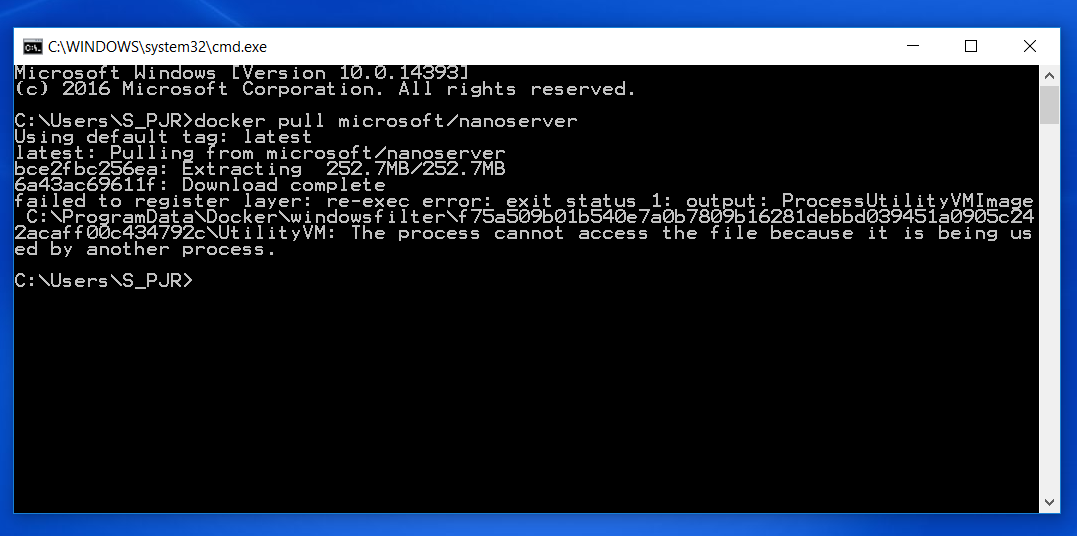
\includegraphics[width=\textwidth,height=\textheight,keepaspectratio]{afbeelding/testCrossContainer/bad_cut.png}
\caption{Error tijdens het gebruiken van Windows Docker containers}
\label{fig:testContainer:crosscontainer}
\end{sidewaysfigure}

\begin{sidewaysfigure}
\centering
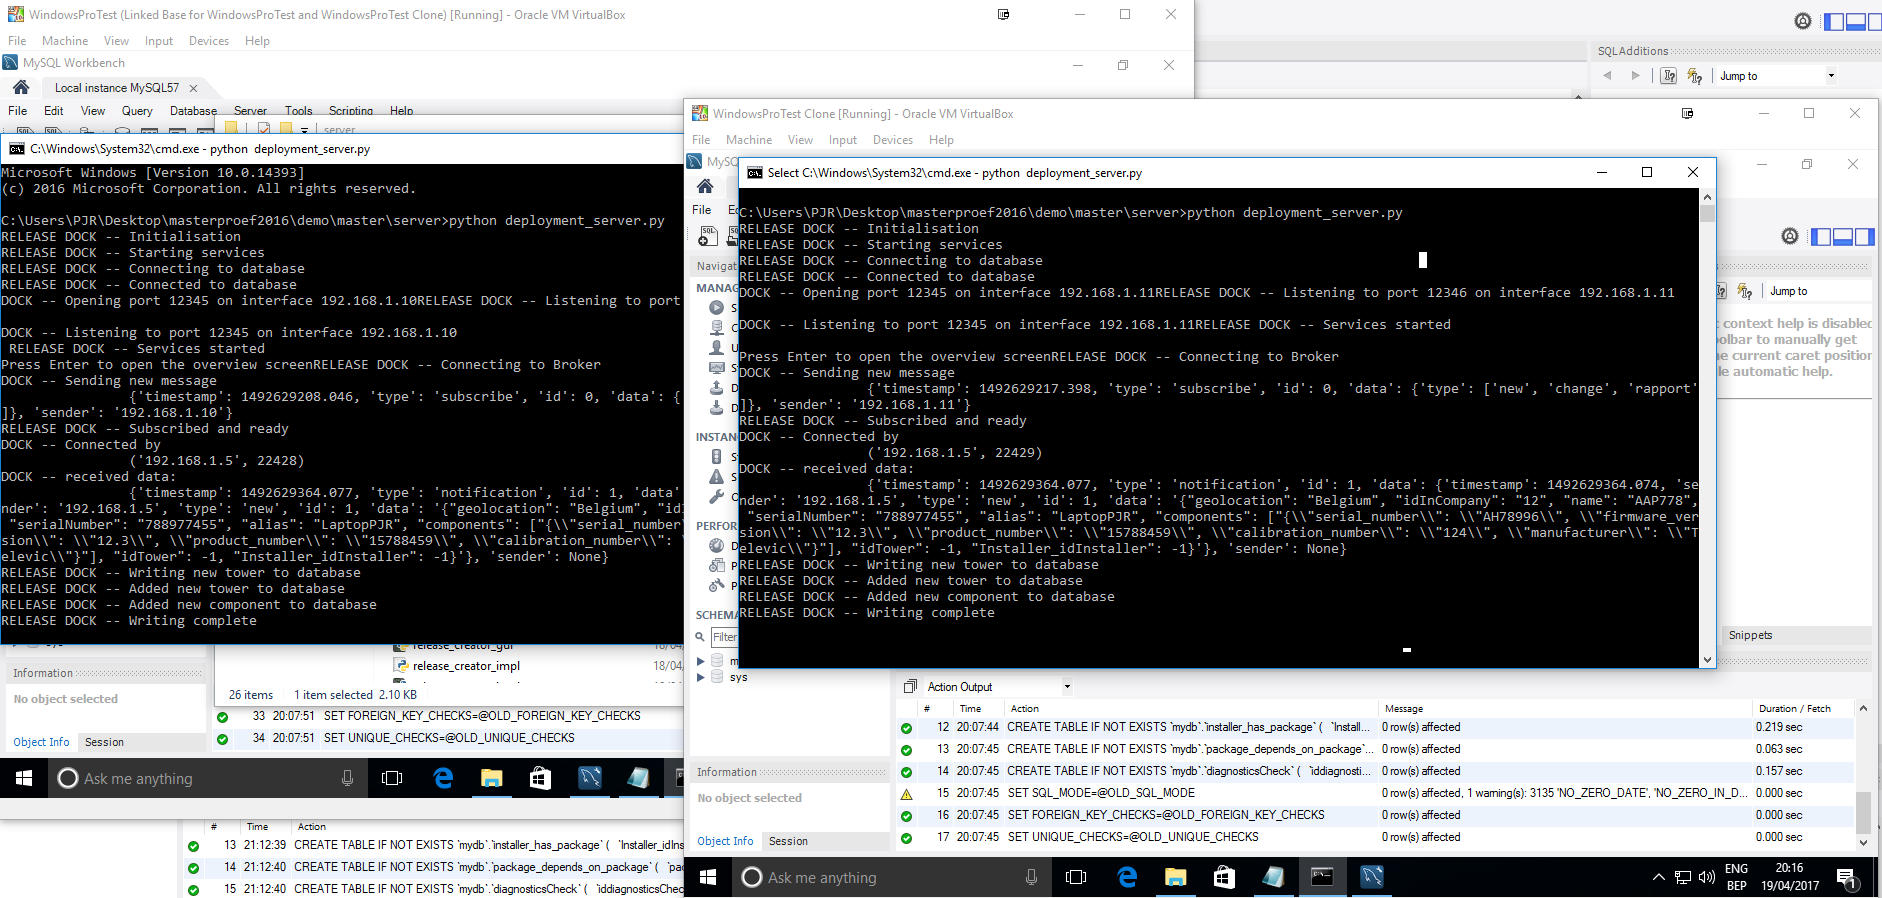
\includegraphics[width=\textwidth,height=\textheight,keepaspectratio]{afbeelding/testMultiServer/receivedSetup.png}
\caption{Ontvangen van client informatie bij servers}
\label{fig:testServer:receiveSetup}
\end{sidewaysfigure}

\subsection{Meerdere servers}
\subsubsection{Doel}
Een volgende test bestaat uit het testen van de functionaliteiten als meerdere servers aanwezig zijn.
Dit gebeurt aan de hand van een virtuele machine met Windows 10.
Iedere virtuele machine bevat de server code samen met een databank om alle gegevens in op te slaan.
De testomgeving bestaat uit drie release docks, één broker en één field dock.

De test bestaat uit het toevoegen van de beschrijving van het field dock aan alle databanken.
Hierna wordt een installer gecreëerd op één van de release docks en wordt deze gereleased.
Het is de bedoeling om in ieder release dock de aanpassing door te voeren.

\subsubsection{Resultaten}
Het eerste deel van de test bestaat uit het toevoegen van de client aan de nodige databanken.
Figuur~\ref{fig:testServer:setup} toont de beschrijving van het field dock weer.
Figuur~\ref{fig:testServer:receiveSetup} geeft weer hoe de beschrijving van het field dock toekomt bij de release docks.
Figuur~\ref{fig:testServer:overview} toont vervolgens de managersinterface van beide release docks.
Hieruit kan afgeleid worden dat ieder release dock de beschrijving correct heeft toegevoegd aan de databank.

Bij het releasen van de installer loopt het echter verkeerd af.
De gereleasde installer komt correct bij de client toe (zie Figuur~\ref{fig:testServer:installation}) en wordt correct geïnstalleerd  maar het verzenden van een update naar de release docks zorgt voor een fout.
De fout die opgegooid wordt, ontstaat doordat het release dock de ID van de installer gaat opvragen in de databank.
Het release dock die de installer heeft aangemaakt, vindt de correcte installer maar de andere release docks vinden deze niet terug in de databank.
Dit komt doordat de informatie van de installer niet doorgegeven wordt aan de verschillende release docks.
De installer komt dus niet in de databank terecht.
In het ontwerp werd hier echter wel rekening mee gehouden.
Deze functionaliteit werd nog niet geïmplementeerd.

De functionaliteit kan op verscheidene manier geïmplementeerd worden.
Zo kan bijvoorbeeld gewerkt worden met maar één databank.
Een andere manier bestaat uit het inschrijven van de release docks bij de broker voor berichten van het type ``release''.
Mocht een notificatie van de broker toekomen met hierin de informatie over een nieuwe installer, dan kan deze gebruikt worden om de installer toe te voegen aan de databank.


\section{SWOT analyse}
\subsection{Strengths}
Het gebruik van de software dock architectuur zorgt voor een schaalbare en flexibele applicatie die de continue toename van gebruikers en software pakketten ondersteunt.
De ontworpen applicatie vormt een goede basis voor Televic om uit te breiden.

Hiernaast zorgt Docker voor een veilige installatieomgeving.
Dit zorgt ervoor dat fouten tijdens het installatieproces geen invloed hebben op het systeem en er altijd een versie van de software van Televic beschikbaar gaat zijn.
%Schaalbaar naar de toekomst toe
%Goed omgaan met verschillende types van installatie

\subsection{Weaknesses}
Een zwakte van de architectuur ligt bij de huidige implementatie van de broker.
Aangezien de broker alle berichten moet afhandelen, vormt deze een bottleneck in de architectuur.
Er zijn echter oplossingen mogelijk waarbij de broker een handle terug geeft aan de docks \citep{adler1995distributed}. 
Een andere strategie bestaat uit het gebruiken van meerdere brokers.

Veiligheid vormt ook een zwakte voor de applicatie.
Het verzenden en ontvangen van berichten gebeurt momenteel niet veilig aangezien alle berichten ongeëncrypteerd verzonden worden.
Dit is echter op te lossen door cryptografische primitieven toe te voegen aan de applicatie.

De voornaamste zwakte bestaat uit het verder vervolledigen van de applicatie.
Naast het installatieproces moet het ook mogelijk zijn om een updateproces uit te voeren.
Hiervoor zijn al enkele methodes aanwezig die gebruikt kunnen worden.

\subsection{Opportunities}
Met de ontworpen architectuur is het mogelijk om verschillende applicaties te verspreiden naar een groep gebruikers.
Dit biedt de mogelijkheid voor Televic om samen te werken met verschillende softwareverkopers om software tussen softwaregebruikers te verspreiden.

\subsection{Threats}
Een bedreiging van de applicatie ligt bij het gebruik van Docker.
Mochten problemen bij de Docker Python module of Docker voor Windows, dan is Televic afhankelijk van een aparte groep van ontwikkelaars die deze problemen zo snel mogelijk moeten oplossen.
%Afhankelijk van de developpers bij Docker om de windows containers te implementeren
%Tijdens ontwerpen heeft het vrijgeven van een windows update alles kapot gemaakt

%geen beveiliging aanwezig

%nog niet volledige communicatie tussen fielddocks aanwezig